\chapter{实验与结果分析}

本章对论文所提方法完成了实验与结果分析。
首先给出了实验设置，包括实验环境、实验用数据集、智能体配置及动作空间，以及实验用评估指标。
然后，与当前已有的各类baseline和SOTA方法进行了对比实验，并给出了实验结果分析。
随后，通过消融实验，评估了本文所提方法中各个组件的有效性，并评估了所提方法的计算效率，最后进行了误差分析。

\section{实验准备}
\subsection{实验环境}
本文使用Hello Robot Stretch平台\cite{hello_robot_stretch_2}开展实验，使用Habitat-sim仿真器\cite{habitat-sim}。
在本地服务器搭建完整的开发环境，保证各阶段实验顺利进行。
\begin{enumerate}
    \item \textbf{硬件环境：}
    本实验使用本地服务器进行训练测试，主要硬件配置如下：
    
    处理器（CPU）：Intel Core i7-14700K
    
    内存（RAM）：32GB
    
    显卡（GPU）：RTX 4090

    \item \textbf{核心软件环境：}
    
    Python：3.9.16

    Pytorch：2.1.1

    CUDA：12.8

    Habitat-sim：0.1.0

\end{enumerate}

\subsection{实验用数据集}
遵从GaussNav原论文，本文在Habitat仿真器\cite{habitat-sim}中使用Habitat-Matterport3D数据集（HM3D）\cite{HM3D}展开实验。
HM3D数据集由真实环境的3D重建场景构成。
目标图所包含的物体实例属于COCO数据类别中的六个，如表\ref{tab:cocoid对应关系表}所示。

% \begin{table}[htbp]
%     \centering
%     \caption{目标图像物体实例对应的COCO类别}
%     \begin{tabular}{ccccccc}
%         \toprule
%         物体类别 & 椅子 & 沙发 & 盆栽植物 & 床 & 马桶 & 电视 \\
%         \midrule
%         对应COCO ID & 56 & 57 & 58 & 59 & 61 & 62 \\
%         \bottomrule
%     \end{tabular}
%     \label{tab:coco_categories}
% \end{table}


\subsection{智能体配置}
遵循GaussNav论文，本文同样采用Hello Robot Stretch\cite{hello_robot_stretch_2}平台的实体化参数。
仿真智能体是一个零转弯半径的刚体圆柱体，高度为1.41米，半径为0.17米，在离地高度1.31米处装有一个前向的RGB-D相机。
在每个时间步$t$，智能体的观测包括以自我为中心的RGB图像、深度图像、目标图像以及传感器位姿读数。
智能体相机与目标相机的规格全部统一为$512\times 512$。
智能体相机使用标准针孔相机模型，水平视场角定义为90度，水平焦距$f_x$计算公式为
\begin{equation}
    f_x=\frac{w}{2\cdot \tan{(\frac{\theta_h}{2})}}
\end{equation}
其中，$\theta_h$是相机在水平方向上能够捕捉到的最大角度，$w$是相机图像的宽度。
垂直焦距$f_y=f_x$。

相机主点，即相机光轴图像平面的交点。
在无畸变的针孔相机中，主点恰好位于图像的中心，计算方式为：
\begin{equation}
    c_x = \frac{w}{2}, \quad c_y = \frac{h}{2}
\end{equation}
其中，$h$是相机图像的高度。

\subsection{智能体的动作空间}
采用离散动作空间进行导航，包含四种动作：\{STOP, FORWARD, TURN\_RIGHT, TURN\_LEFT\}。
STOP动作会停止当前任务回合；
FORWARD动作会在每个时间步内使智能体向前移动25cm；
TURN\_RIGH和TURN\_LEFT动作会使智能体在原地顺时针或者逆时针旋转25度。

\subsection{评估指标}
在高斯渲染阶段，除了使用原始3DGS使用的SSIM、PSNR、RMSE、L1和LPIPS指标来评估RGB重建质量外，本文还针对高斯语义渲染质量引入了DICE系数和Focal IoU系数来评估语义渲染质量。
原GaussNav论文中并没有针对语义渲染情况做出评估，因此本文也对比了语义是否参与监督与优化的渲染质量。

同时，遵循krantz等人\cite{krantz2023navigating}的方法，本文使用导航成功率（Success）以及归一化逆路径长度（SPL）\cite{anderson2018evaluation}作为成功率和效率的评估指标。
当智能体调用STOP动作时，系统判定智能体目前所在位置和目标位置的直线欧式距离是否小于等于1米，若小于1米则判定成功$Success=1$，否则判定失败$Success=0$。

$SPL$具体计算公式为：
\begin{equation}
    SPL=\frac{1}{N}\sum _{i=1}^{N}S_{i}\cdot \frac{l_i}{max(p_i,l_i)}
\end{equation}

其中$N$为任务回合总数，$S_i$为第$i$个任务回合的二值成功指示符号，$l_i$为从起始位置到目标的最短路径距离，$p_i$为智能体实际走过的路径长度。
$SPL$值越高，表示导航效率越高。



\section{与现有方案的对比}
为证明论文所提方法的有效性，本文选取了领域内多种baseline方法以及先进方法进行了对比实验。
其中，Baseline方法包括了RL Baseline\cite{krantz2022instance}和OVRL-v2\cite{yadav2023ovrl}，先进方法包括了Mod-II\cite{krantz2023navigating}，SOTA方法包括了GaussNav\cite{gaussnav}。
为确保实验公平性，所有实验均在相同的 HM3D 验证集（包含36个场景、1000个测试任务）、场景特定地图设置和硬件环境下进行。
对比结果如表格\ref{tab:hm3d_performance}所示。
% 导航方法的对比表格
\begin{table}[htbp]
\centering
\caption{与现有导航方案的对比}
\begin{tabular}{lcc}
\toprule
对比方法 & Success $\uparrow$ & SPL $\uparrow$ \\
\midrule
RL Baseline \cite{krantz2022instance} & 0.083 & 0.035 \\
OVRL-v2 \cite{yadav2023ovrl}  & 0.006 & 0.002 \\
% OVRL-v2 IIN \cite{yadav2023ovrl} & 0.248 & 0.118 \\
% FGPrompt \cite{sun2023fgprompt} & 0.099 & 0.028 \\
% \midrule
% MultiON Baseline \cite{51} & 0.066 & 0.045 \\
% MultiON Implicit \cite{53} & 0.143 & 0.107 \\
% MultiON Camera \cite{50} & 0.186 & 0.142 \\
% \midrule
% Mod-IIN \cite{20} & 0.561 & 0.233 \\
% IEVE Mask RCNN \cite{22} & 0.684 & 0.241 \\
% IEVE InternImage \cite{22} & 0.702 & 0.252 \\
\midrule
% Mod-II\cite{krantz2023navigating} & 0.561 & 0.233\\
Mod-II\cite{krantz2023navigating} & 0.573 & 0.313 \\
% IEVE Mask RCNN \cite{lei2024instance} (Scene Map) & 0.684 & 0.334 \\
% IEVE InternImage \cite{lei2024instance} (Scene Map) & 0.693 & 0.322   \\
\midrule
GaussNav \cite{gaussnav} & 0.725 & 0.578 \\
\textbf{GSGuide (Ours)} & \textbf{0.778} & \textbf{0.585} \\
\bottomrule
\end{tabular}
\label{tab:hm3d_performance}
\end{table}



一方面，传统的实例目标图像导航会在每一个episode中重新生成场景地图。
不同的是，本文所提出的框架会为同一个场景构建一个可以复用的地图。
表格中第一部分呈现了几种基线方法，第二部分对比了本文所提出的框架与SOTA方法(包括GaussNav\cite{gaussnav})在本文所使用的特定场景数据集上的性能对比。
% 结果的一个分析

\subsection{端到端baseline方法}
本文评估了两种代表性的端到端方法在 IIN 任务上的性能。

\textbf{RL Baseline}\cite{krantz2022instance}构建了一个端到端的强化学习网络，该网络直接接收智能体的 RGB 图像、深度图像、目标图像、GPS 坐标和航向角作为输入，通过独立的视觉编码器和位置编码器提取特征，经两层 LSTM 融合后输出动作决策。
该网络使用近端策略优化（PPO）算法从头开始训练，最终仅取得了 0.083 的成功率和 0.035 的 SPL。
这一结果表明，纯端到端的强化学习框架难以同时掌握 IIN 任务所需的场景语义理解、跨视角实例识别和长期空间记忆等核心能力，导致导航性能和效率均处于较低水平。

\textbf{OVRL-v2}\cite{yadav2023ovrl}是当前图像目标导航（ImageGoal Navigation）任务的代表性基线方法，其核心是通过自监督预训练学习通用的视觉表示。
本文将在 ImageGoal 任务上预训练的 OVRL-v2 模型应用于 IIN 任务，发现其性能极差，成功率仅为 0.006，远低于基于地图的模块化方法。
这一显著的性能下降主要源于三个方面的不匹配：一是场景数据集从 Gibson\cite{xia2018gibson} 切换到了 HM3D，二是机器人本体从 Locobot\cite{locobot_official_website} 变为了Hello Robot Stretch\cite{hello_robot_stretch_2}，三是任务目标从 "导航到图像拍摄位置" 转变为 "导航到图像中的特定物体实例"。
这进一步验证了端到端方法在处理需要精细实例区分和空间推理的 IIN 任务时存在固有局限性。

\subsection{先进方法对比}
本文评估了当前 IIN 任务的先进方法，并统一使用场景特定地图（Scene Map）设置进行公平对比。
场景特定地图允许智能体在同一场景的不同导航回合中复用预先构建的地图，避免了重复探索的开销，这也是本文方法采用的实验设置。

\textbf{Mod-IIN}\cite{krantz2023navigating}是一个系统性解决 IIN 任务的模块化方法，它将任务分解为探索、目标实例重识别、目标定位和局部导航四个独立子任务，每个子任务均使用无需微调的现成组件实现。
将模型应用于本文所使用的HM3D数据集进行测试，结果表明Mod-IIN 的$SPL$达到了 0.313，成功率达到 0.573，这表明基于地图的模块化方法在 IIN 任务中具有较大优势。

\subsection{SOTA对比}
\textbf{GaussNav}\cite{gaussnav}通过引入 3D 高斯溅射技术构建语义高斯地图，实现了 IIN 任务性能显著提升。
与传统 BEV 地图仅能保留 2D 几何和粗粒度语义信息不同，语义高斯地图同时编码了场景的 3D 几何结构、每个高斯的语义标签以及物体的精细纹理特征。
这使得智能体能够直接从地图中渲染出物体实例的多视角（NVS）描述性图像，与目标图像进行特征匹配从而精确确定目标实例与目标位置，无需像 BEV 地图方法那样对潜在候选对象进行额外的近距离验证。
实验结果显示，GaussNav 在场景特定地图设置下取得了 0.725 的成功率和 0.578 的 SPL，充分证明了语义高斯地图表示在实例级导航任务中的显著优势。

本文提出的 GSGuide 方法在 GaussNav 的基础上，通过两个关键创新进一步提升了导航性能：
\begin{enumerate}
\item \textbf{语义渲染监督机制：}通过为每个高斯引入可训练的语义向量，并在优化过程中持续监督语义渲染质量，解决了原始 GaussNav 中语义标签与几何纹理参数脱节的问题。这使得语义高斯地图能够更准确地编码场景的细粒度语义信息，提升了实例级目标识别的可靠性。
\item \textbf{位姿精修 Warping Loss：}通过最小化渲染图像与目标图像之间的像素级光度损失，实现了亚像素级的位姿优化。这种稠密对齐方式能够有效修正基于稀疏特征匹配得到的初始位姿偏差，特别适用于纹理较少或存在遮挡的场景。
\end{enumerate}

实验结果表明，GSGuide 的导航成功率从 GaussNav 的 0.725 提升至 0.778（相对提升 7.31\%），同时 SPL 从 0.578 提升至 0.585（相对提升 1.21\%）。
这一结果验证了两个核心改进的有效性：
语义渲染监督机制主要提升了目标识别的准确性，而位姿精修 Warping Loss 则优化了目标定位的精度。两者协同作用，使 GSGuide 在 HM3D 数据集上取得了当前最优的导航性能。

% 如图\ref{fig:after_optimization}所示，含有不同语义信息的实例物体我们选用了不同的颜色进行可视化。
% \begin{figure}
% \centering
% 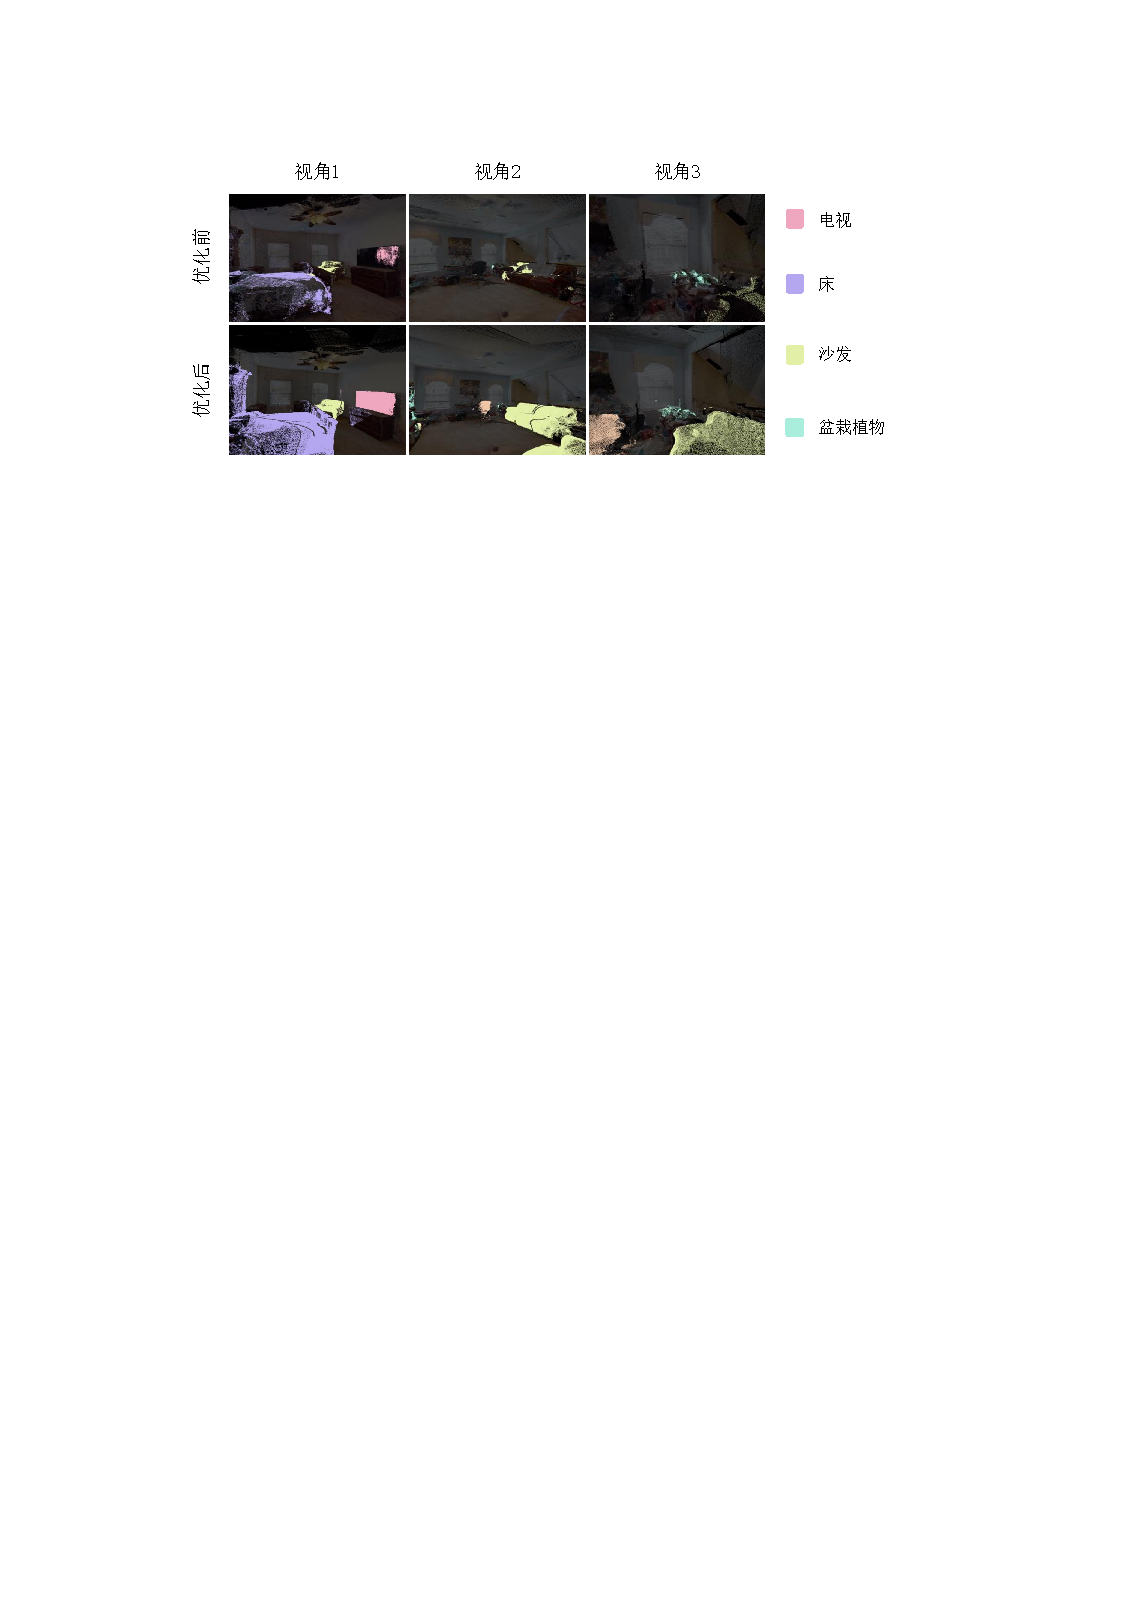
\includegraphics[width=1.0\textwidth]{figures/图标ppt/语义优化前后对比图.pdf}
% \caption{语义渲染监督机制优化前后对比}
% \label{fig:after_optimization}
% \end{figure}

% 我们选取了三个视角进行对比，可以明显看出，相较于优化前优化后高斯覆盖更加完整、连续，物体表面覆盖断层减少，这为导航点计算提供了更准确的参考。


\section{消融实验}
\subsection{消融实验设置与结果}
为了系统验证本文提出的语义渲染监督机制和位姿精修 Warping Loss两个核心改进的有效性，本文设计了三组对照消融实验。

\begin{table}[htbp]
\centering
\caption{消融实验导航性能结果}
\begin{tabular}{lcccc}
\toprule
消融实验设置 & Success$\uparrow$ & $\Delta$Success & SPL$\uparrow$ & $\Delta$SPL \\
\midrule
GSGuide & 0.778 & -- & 0.585 & -- \\
GSGuide w.o. Supervised Segmentation & 0.723 & -0.055 & 0.577 & -0.008 \\
GSGuide w.o. Warping loss & 0.748 & -0.030 & 0.582 & -0.003 \\
\bottomrule
\end{tabular}
\label{tab:ablation_study}
\end{table}

\begin{table}[htbp]
\centering
\caption{消融实验语义渲染指标结果}
\begin{tabular}{lccc}
\toprule
消融实验设置 & 交叉熵损失$\downarrow$ & Dice损失$\downarrow$ & Focal IoU损失$\downarrow$ \\
\midrule
GSGuide & 1.501 & 0.867 & 0.915 \\
GSGuide w.o. Supervised Segmentation & 1.801 & 0.891 & 0.971 \\
GSGuide w.o. Warping loss & 1.501 & 0.867 & 0.915 \\
\bottomrule
\end{tabular}
\label{tab:ablation_semantic}
\end{table}

\subsection{语义渲染监督有效性}
本实验移除了本文提出的语义渲染监督机制，即完全遵从原始 GaussNav 的语义处理流程：仅在高斯初始化阶段通过 Mask R-CNN 的分割结果为每个高斯分配一次性静态语义标签，在后续的可微渲染优化和高斯致密化过程中禁用语义标签梯度跟踪，不再引入任何语义损失进行监督，仅保留原始 3DGS 的 RGB 和深度重建损失。

导航性能的消融实验结果如表 \ref{tab:ablation_study} 所示，移除语义渲染监督后，模型的成功率从 0.778 下降至 0.723，相对下降幅度为 7.07\%；SPL 从 0.585 小幅下降至 0.577，相对下降幅度为 1.37\%。

语义渲染指标如表 \ref{tab:ablation_semantic} 所示，移除监督后交叉熵损失从 1.501 上升至 1.801，相对上升 20.0\%；Dice 损失从 0.867 上升至 0.891，相对上升 2.8\%；Focal IoU 损失从 0.915 上升至 0.971，相对上升 6.1\%。

深入分析表明：
\begin{enumerate}
    \item \textbf{语义错位问题}：静态语义标签并不会跟随高斯的3D几何纹理参数同步更新，在多轮迭代优化后，高斯的位置、大小可能发生变化，但语义标签保持不变，导致语义错位问题，进而引起物体边界模糊、覆盖不完整不连续等问题。
    
    \item \textbf{误差传递效应}：语义误差会传递到后续的实例匹配阶段。由于语义标签不准确，在检索相同类别的候选物体时可能会遗漏真正的目标，或者引入无关的干扰物体，导致物体实例匹配得分受到影响，进而引发部分目标匹配混淆。
    
    \item \textbf{对SPL的有限影响}：SPL的小幅度下降说明语义渲染监督主要影响目标识别的准确性，对于已经确定的目标实例，后续的导航路径规划效率受到的影响较小。这是因为路径规划主要依赖场景的几何结构，而非精细的语义信息。
\end{enumerate}

进一步分析发现，移除语义渲染监督后的模型性能（0.723/0.577）与原始 GaussNav（0.725/0.578）几乎完全持平，性能差异小于 0.3\%，在统计上不显著。这一对照结果严格证明：语义渲染监督是本文方法相对于 GaussNav 的核心性能提升来源，其他实验设置（如相机参数统一、训练超参数调整）对最终结果的影响可以忽略不计。

为进一步展现语义监督机制的有效性，本文可视化对比了语义参与监督前后的渲染效果。
如图\ref{fig:after_optimization}所示，含有不同语义信息的实例物体本文选用了不同的颜色进行可视化。
\begin{figure}
\centering
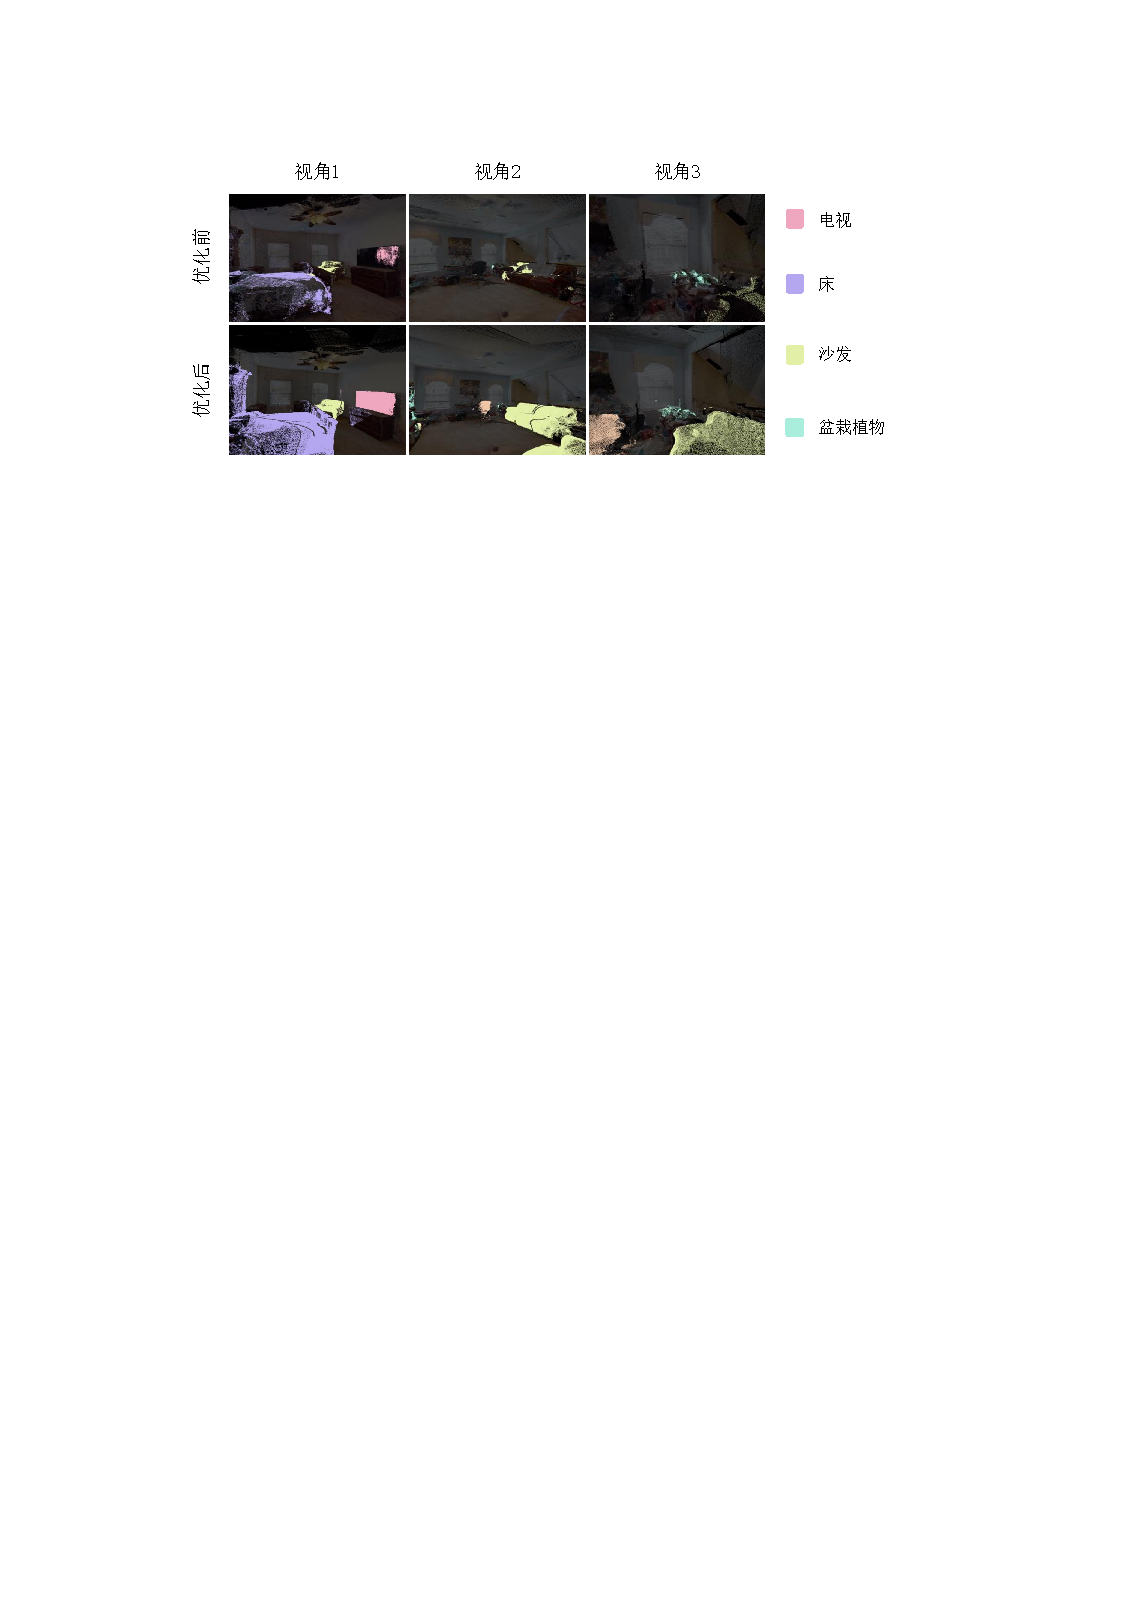
\includegraphics[width=1.0\textwidth]{figures/图标ppt/语义优化前后对比图.pdf}
\caption{语义渲染监督机制优化前后对比}
\label{fig:after_optimization}
\end{figure}

本文选取了三个视角进行对比，可以明显看出，相较于优化前优化后高斯覆盖更加完整、连续，物体表面覆盖断层减少，这为导航点计算提供了更准确的参考。


\subsection{位姿精修Warping Loss有效性}
本实验移除了本文提出的位姿精修 Warping Loss 模块，即在目标匹配阶段仅使用 DISK+LightGlue 的特征匹配结果直接估算目标的 3D 位置，不再通过光度对齐损失对目标的位姿进行精细化优化。

导航性能结果如表 \ref{tab:ablation_study} 所示，移除 Warping Loss 后，模型的成功率从 0.778 下降至 0.748，相对下降幅度为 3.86\%；SPL 从 0.585 下降至 0.582，相对下降幅度为 0.51\%。

语义渲染指标如表 \ref{tab:ablation_semantic} 所示，移除 Warping Loss 后各项指标保持不变，因为位姿精修模块与语义优化在流程上处于前后两个阶段，是完全独立的两个环节，因此移除位姿精修模块对语义渲染质量没有影响，主要作用于位姿优化阶段。

深入分析表明：
\begin{enumerate}
    \item \textbf{特征匹配的局限性}：传统的局部特征匹配方法主要基于稀疏关键点估算目标的位置，对于纹理较少的物体（如光滑的墙壁、白色家具）或存在部分遮挡的物体，可用的关键点数量大幅减少，容易引起较大的定位偏差。
    
    \item \textbf{光度对齐的优势}：本文引入 warping loss 最小化渲染图像与目标图像之间的像素级光度损失，能够使相机位姿尽可能优化到目标图像拍摄位姿。相比于仅使用稀疏特征匹配，这种稠密对齐方式显著提升了定位准确性。

\end{enumerate}

SPL 的微小变化同样说明，位姿精修主要影响目标定位的精度，只要能够正确识别目标并确定其大致位置，导航路径的长度不会发生显著变化。

\subsection{消融实验结论}
消融实验结果充分验证了本文提出的两个核心改进的有效性，通过定量分析可以得出以下结论：

\begin{itemize}
    \item \textbf{语义渲染监督}是性能提升的主要来源，贡献了 7.07\% 的成功率提升，同时显著改善了所有语义渲染指标（交叉熵损失下降 20.0\%，Dice 损失下降 2.8\%，Focal IoU 损失下降 6.1\%），解决了原始 GaussNav 中语义标签与几何纹理脱节的问题；
    
    \item \textbf{位姿精修 Warping Loss} 贡献了 3.86\% 的成功率提升，进一步优化了目标定位的精度，但对语义渲染质量几乎没有影响；
    
    \item 两个模块具有良好的协同效应，联合使用时取得了最佳性能；
    
    \item 语义渲染监督主要影响目标识别阶段，而位姿精修 Warping Loss 主要影响目标定位阶段，两者作用于不同环节，形成互补。
\end{itemize}

两者协同作用使本文方法在 HM3D 数据集上均取得了优于 GaussNav 的性能。

\section{误差分析}
本文提出的 GSGuide 框架仍然有提升空间。
为了明确未来的改进方向，本文分析了框架的主要误差来源。
具体而言，误差主要来自于语义错误识别和场景建立质量不完善两个方面：

\subsection{语义错误识别}
前期语义分割依赖于Yolo26语义分割模型，在某些场景中存在一定的误识别。
具体而言，Yolo26有时会将一个物体归为错误的语义类别。
例如图\ref{fig:语义估计错误导致位姿估计错误}所示，
\begin{figure}
    \centering
    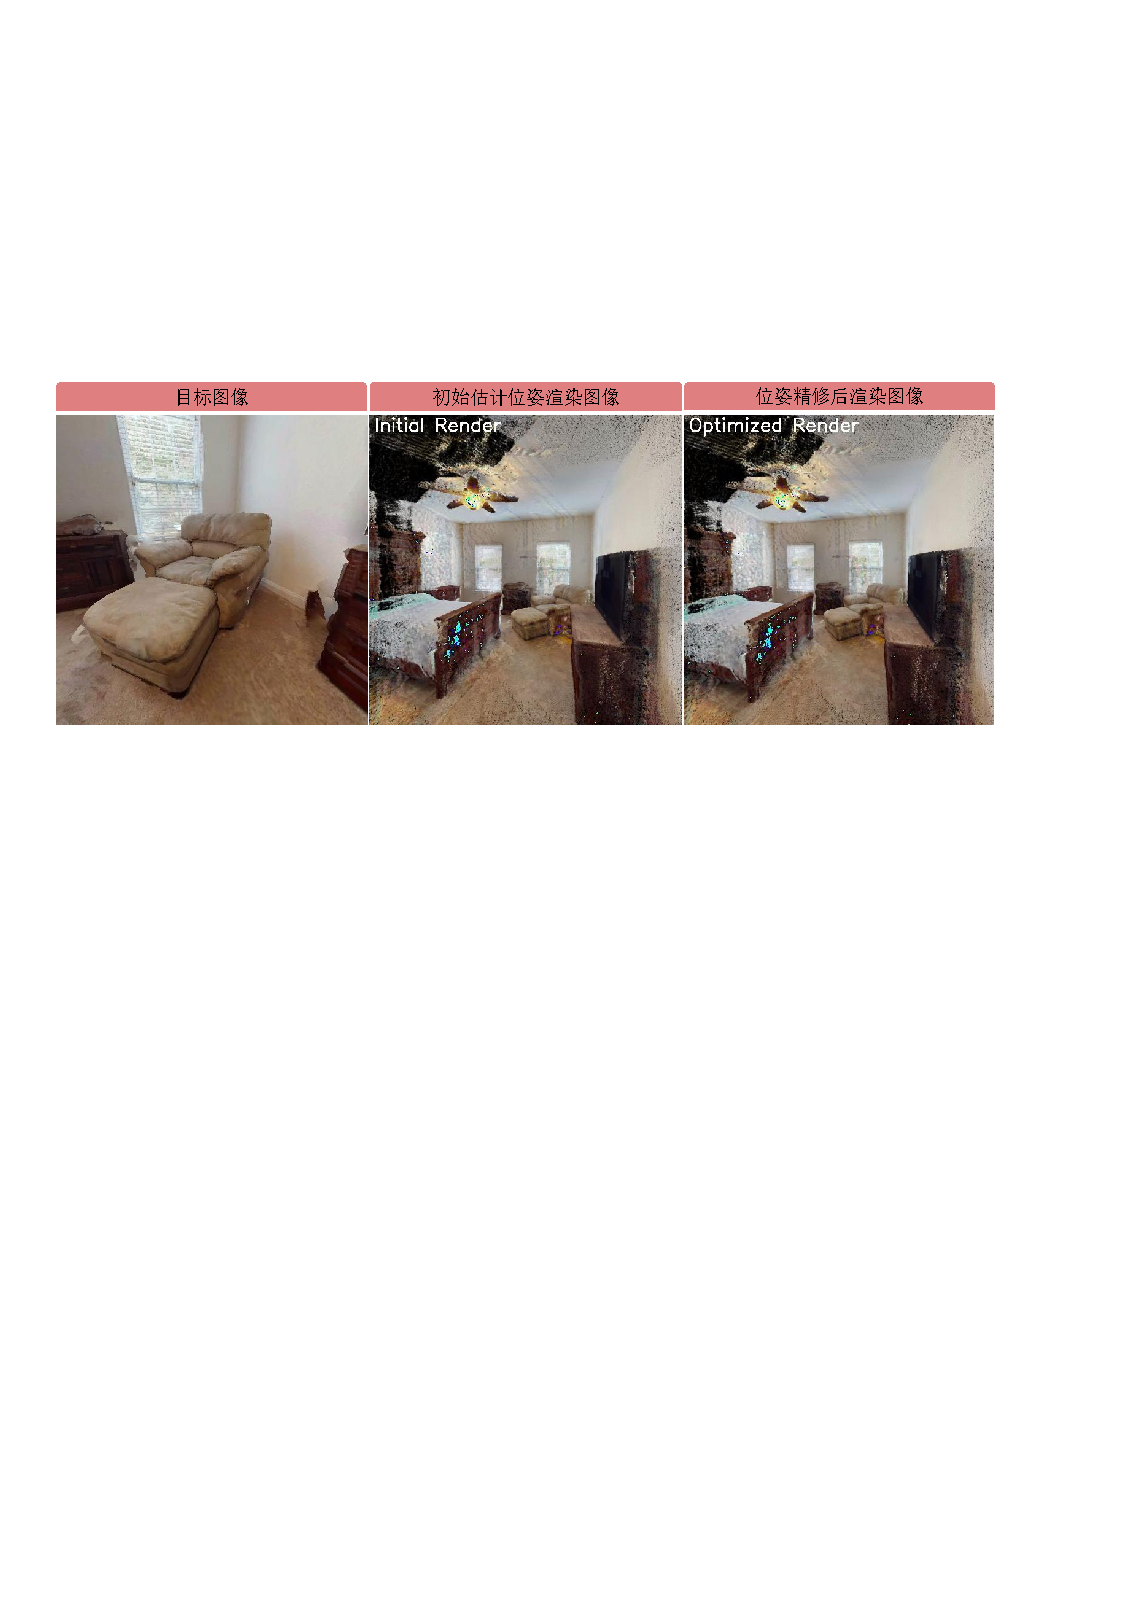
\includegraphics[width=1.0\textwidth]{figures/图标ppt/语义估计错误导致目标估计失败.pdf}
    \caption{语义信息错误导致位姿错误估计}
    \label{fig:语义估计错误导致位姿估计错误}
\end{figure}
目标图像的 GT COCO ID 被标记为56（椅子），而Yolo26却将其归为59（床），进而在初始位姿估计时出现严重偏差，导致可导航点计算失败。

\subsection{场景建立质量不完善}
如表\ref{tab:场景构建质量量化}所示，
\begin{table}[htbp]
\centering
\caption{场景构建质量}
\begin{tabular}{ccccc}
\toprule
Avg. PSNR $\uparrow$ &Avg. RMSE$\downarrow$ &Avg. L1$\downarrow$ & Avg. MS-SSIM$\uparrow$ & Avg. LPIPS$\downarrow$ \\
\midrule
29.71 & 4.75 & 4.75 & 0.966 & 0.176 \\
\bottomrule
\end{tabular}
\label{tab:场景构建质量量化}
\end{table}
尽管本文提出的GsGuide框架展现出良好的综合重建性能，其平均峰值信噪比（PSNR）达到 29.71 dB，深度估计的均方根误差（RMSE）与平均绝对误差（L1）均为 4.75 cm，表明深度估计精度较高且误差分布均匀无显著离群值；
同时，平均多尺度结构相似性指数（MS-SSIM）高达 0.966，平均感知图像块相似度（LPIPS）低至 0.176，说明重建结果在结构纹理一致性和人眼视觉感知质量方面均和HM3D场景高度一致，但因HM3D场景构建本身存在一定的质量不佳问题，会一定程度上影响后续的目标点计算和导航过程。

具体而言，在将优化后位姿观察所得到的高斯体素化转为2DBEV网格时，会出现可导航点计算错误的情况。
可导航点的估计高度依赖于HM3D场景数据集的构建质量，当场景中存在物体遮挡、场景建立质量不完善等问题时，物体3D边界框会受到严重影响，进而影响后续可导航点计算环节。
如图\ref{fig:场景出现漏洞}红框部分，
\begin{figure}
    \centering
    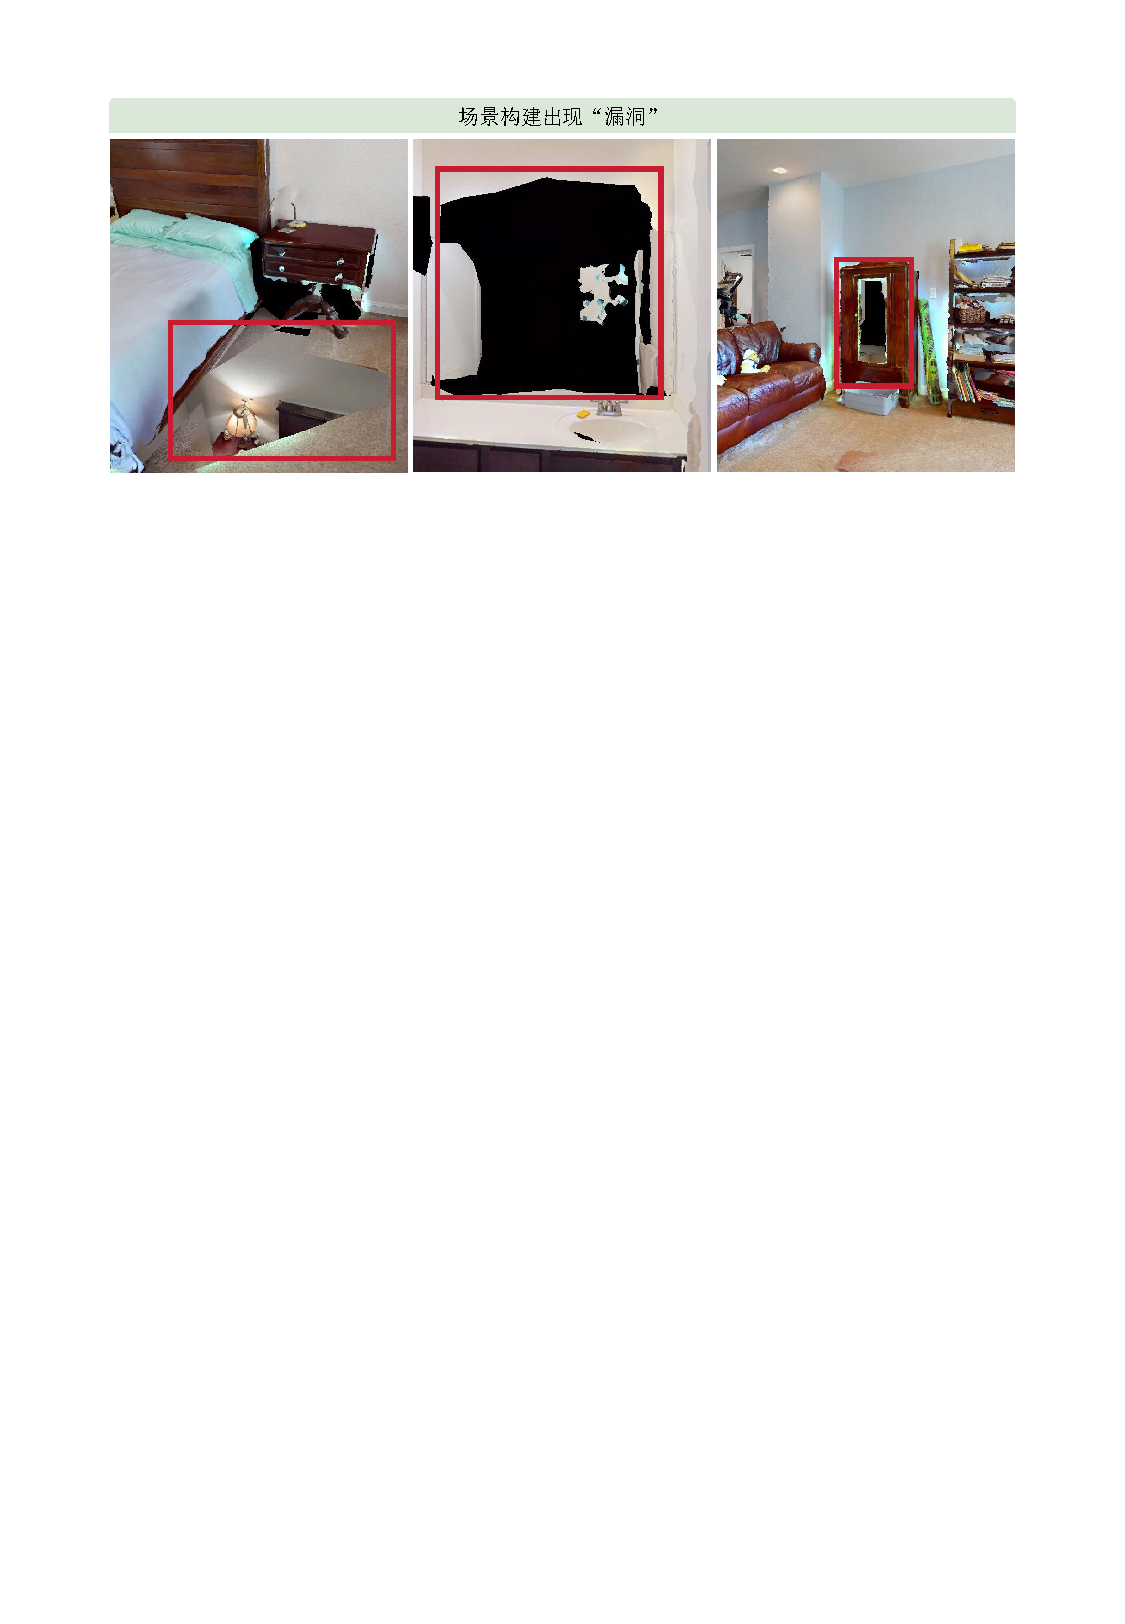
\includegraphics[width=1.0\textwidth]{figures/图标ppt/漏洞.pdf}
    \caption{场景“漏洞”}
    \label{fig:场景出现漏洞}
\end{figure}
因为场景构建质量不完善导致部分实例或者地面等出现“漏洞”，这在某些情况下会导致可导航点无法计算。例如图中的因床左侧地面出现“漏洞”，系统会在体素化时不考虑地面可通行区域，从而忽略该区域的可导航点计算。

又如图\ref{fig:语义信息缺失}红框所示，
\begin{figure}
    \centering
    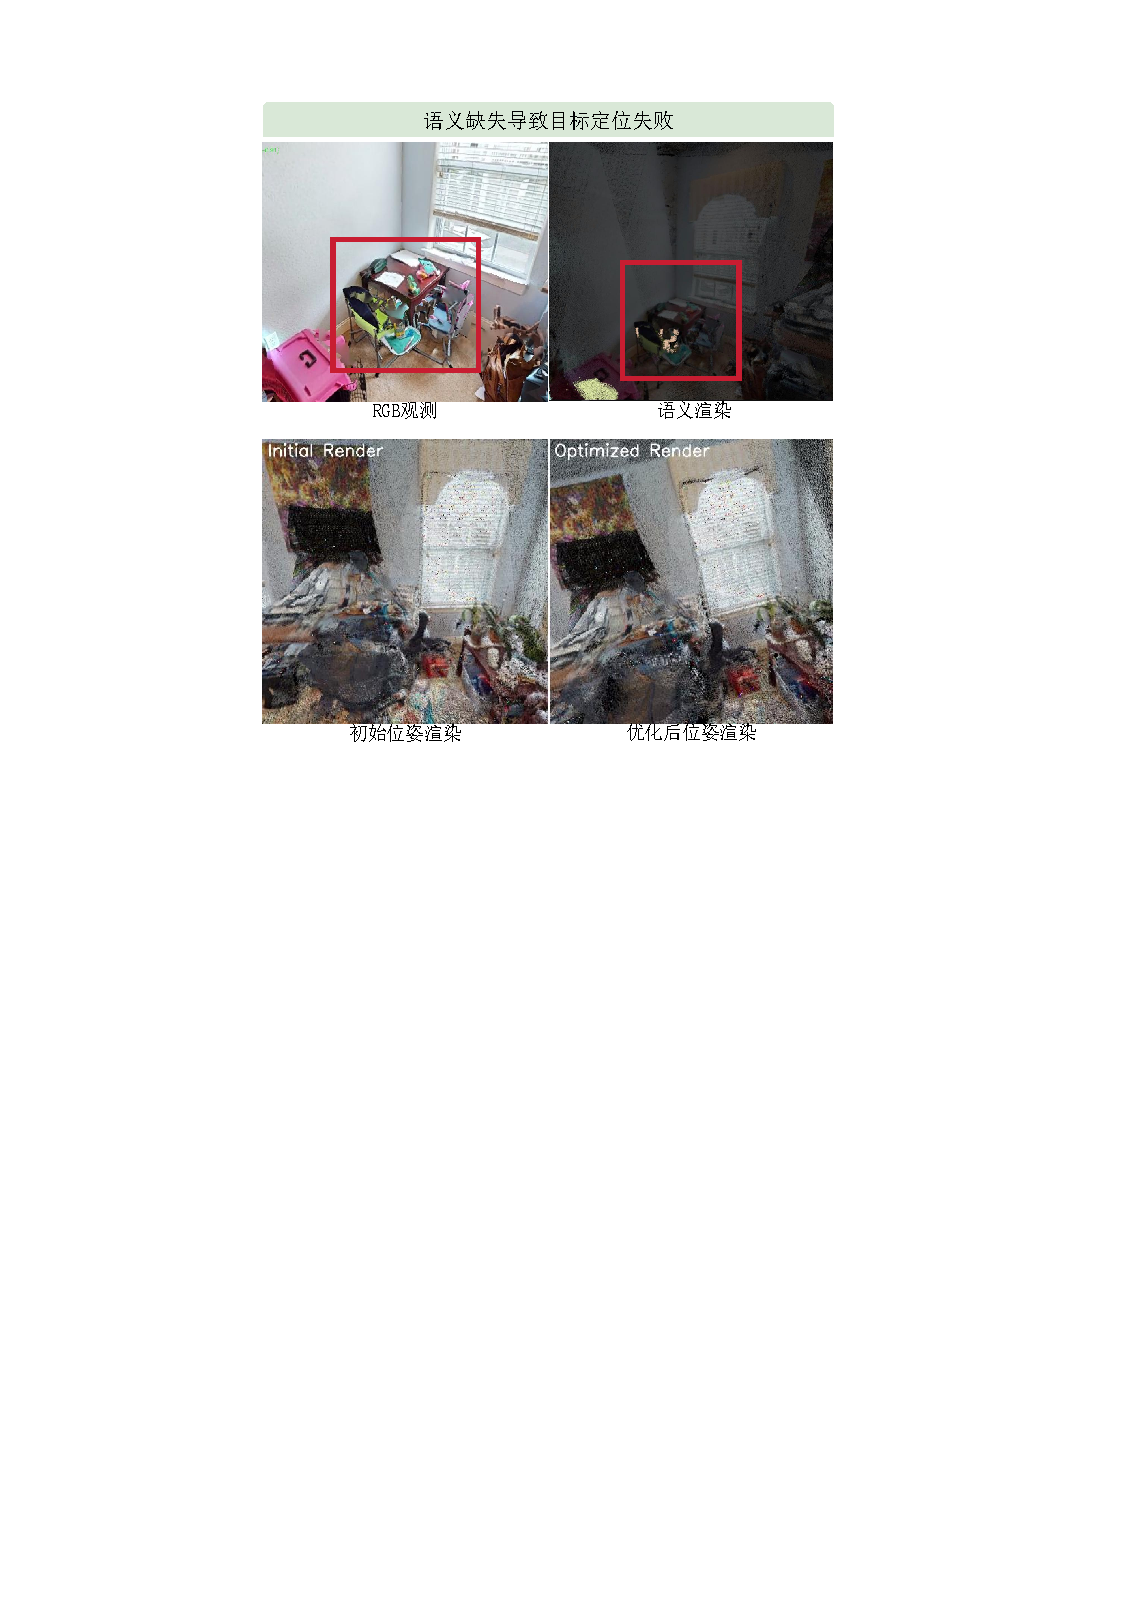
\includegraphics[width=0.6\textwidth]{figures/图标ppt/语义缺失导致目标定位失败.pdf}
    \caption{实例缺失语义信息}
    \label{fig:语义信息缺失}
\end{figure}
HM3D场景数据集的构建质量不佳使得Yolo26无法识别到实例“椅子”，导致这部分语义缺失，初始位姿匹配出现严重偏差，后续的位姿精修则更类似于随机过程。
